\documentclass[12pt]{article}
\usepackage[T1]{fontenc}
\usepackage[french]{babel}
\usepackage{datetime}
\usepackage{subcaption}
\usepackage[letterpaper, margin=1.9cm]{geometry}
\usepackage{graphicx}
\usepackage{epstopdf}
\usepackage{siunitx}
\sisetup{output-decimal-marker = {,}}
\graphicspath{ {../figures} }
\usepackage{derivative}
\usepackage{booktabs}
\usepackage[flushleft]{threeparttable}
\usepackage{amsmath}
\usepackage{parskip}

\usepackage{csquotes}
\usepackage[
backend=biber,
style=ieee,
%style=verbose,
citestyle=ieee,
%sorting=nyt,
%url=false
]{biblatex}
\bibliography{references}

\title{MEC6616 --- TPP2}


\author{Aurélie Grebe\\Noémie Herbinière}
\newdate{duedate}{12}{10}{2026}
\date{\displaydate{duedate}}

\begin{document}
\maketitle

\section{Introduction}

Dans la présente œuvre, nous proposons une résolution de l'équation de convection-diffusion
de la chaleur par volumes finis en 2D. Après une brève explication de
la méthode de résolution, nous analyserons les résultats à l'aide de différents maillages ainsi que pour différents nombres de Peclet.

\section{Méthodologie}

L'équation de convection-diffusion stationnaire est la suivante:
\begin{equation} 
\frac{\partial {(uT)}}{\partial x} + \frac{\partial {(vT)}}{\partial y} - k \left(\frac{\partial^2 {T}}{\partial^2 x} + \frac{\partial^2 {T}}{\partial^2 y} \right) = S
\end{equation}

L'équation est exprimée en forme matricielle par: $A\phi = B$

Avec $A$ contenant les coefficients de diffusion et convection, $\phi$ le champ que l'on souhaite résoudre et $B$ contenant les termes de source et de cross-diffusion.

\subsection{Cellules intérieures}

En méthode centrée:

\begin{align}
	A[T_g,T_g] + &= D_i + \frac{F_i}{2}\\
	A[T_d,T_d] + &= D_i - \frac{F_i}{2}\\
	A[T_g,T_d] + &= -D_i + \frac{F_i}{2}\\
	A[T_d,T_g] + &= -D_i - \frac{F_i}{2}\\
	B[T_g] + &= S_{DC,i} \\
	B[T_d] + &= -S_{DC,i}
\end{align}

En méthode Upwind:

\begin{align}
	A[T_g,T_g] + &= D_i + max(F_i,0)\\
	A[T_d,T_d] + &= D_i + max(-F_i,0)\\
	A[T_g,T_d] + &= -D_i - max(-F_i,0)\\
	A[T_d,T_g] + &= -D_i - max(F_i,0)\\
	B[T_g] + &= S_{DC,i} \\
	B[T_d] + &= -S_{DC,i}
\end{align}

Avec:

\begin{align}
	D_i &= \frac{\Gamma}{P_{NKSI}} \frac{\Delta A_i}{\Delta \xi} \\
	S_{DC,i} &= -\Gamma \left(\frac{P_{KSIETA}}{P_{NKSI}}\right) \left(\frac{\overrightarrow{\mathrm{grad}} \phi_A + \overrightarrow{\mathrm{grad}} \phi_P}{2}\right) \Delta A_i . \hat{e_{\eta}} \\
	F_i = \hat{n_i}.(\rho \overrightarrow{u_i}) \Delta A_i
\end{align}

où:

\begin{align}
	P_{NKSI} &= \hat{n_i}.\hat{e_{\xi}} \\
	P_{KSIETA} &= \hat{e_{\xi}}.\hat{e_{\eta}} \\
	\Delta A_i &= \sqrt{(X_b-X_a)^2+(Y_b-Y_a)^2} \\
	\Delta \eta &= \Delta A_i \\
	\Delta \xi &= \sqrt{(X_A-X_P)^2+(Y_A-Y_P)^2} \\
	e_{\xi} &= \left(\frac{X_A-X_P}{\Delta \xi}, \frac{Y_A-Y_P}{\Delta \xi}\right) \\
	e_{\eta} &= \left(\frac{X_b-X_a}{\Delta \eta}, \frac{Y_b-Y_a}{\Delta \eta}\right)
\end{align}

Ici, $(Xa, Y_a)$ et $(X_b,Y_b)$ sont, respectivement, les coordonnées du premier et deuxième noeud de chaque arrête $i$ tandis que $(X_P,Y_P)$ et $(X_A,Y_A)$ sont les coordonnées des centres de, respectivement, l'élément de gauche et l'élément de droite de l'arrête $i$.

Pour prendre en compte le terme source, on ajoute: $B = B+S_{\phi}A$, où $S_{\phi}$ est le vecteur contenant la valeur du terme source au centre de chaque élément et A le vecteur de leurs aires respectives.

Le calcul de $S_{DC,i}$ nécessitant de connaître le gradient du champ aux points A et P, il faut itérer la résolution plusieurs fois en commençant par $S_{DC,i}=0$. A chaque itération, le $S_{DC,i}$ est re-caclulé en utilisant la méthode Least-Square pour obtenir les gradients provenant du champ $\phi$ obtenu à l'itération précédente. La valeur de la matrice B finit par converger.

\subsection{Cellules aux frontières}

Pour une condition aux limites de Neumann:

En centré:
\begin{align}
A[T_g,T_g] + &= F_i/2 \\
B[T_g] + &= \Gamma \phi'_N \Delta A_i + \frac {F_i \phi'_N P_{NKSI,i} \Delta \xi}{2}
\end{align}

En Upwind:
\begin{align}
A[T_g,T_g] + &= max(F_i,0) \\
B[T_g] + &= \Gamma \phi'_N \Delta A_i + min(F_i,0) \phi'_N P_{NKSI,i} \Delta \xi
\end{align}

Où $\phi'_N$ est la valeur de la condition sur la frontière.

Pour une condition de Dirichlet:

En centré :
\begin{align}
A[T_g,T_g] + &= D_i + F_i/2\\
B[T_g] + &= \phi_D D_i + S_{DC,i} - \phi_D F_i/2
\end{align}

En Upwind:
\begin{align}
A[T_g,T_g] + &= D_i + max(F_i,0)\\
B[T_g] + &= \phi_D D_i + S_{DC,i} + max(-F_i,0) \phi_D
\end{align}

Cependant, attention, les valeurs de $D_i$ et $F_i$ à la frontière changent légèrement pour utiliser la distance selon l'axe $\xi$ entre le centre de l'élément et le milieu de l'arrête frontière. $\phi_D$ est la valeur de la condition sur la frontière. Dans le cas d'une condition de Dirichlet constante, le terme $S_{DC,i}$ est constant.

\subsection{Maillages}

Les cas présentés dans cette œuvre ont été calculé avec des maillages
quadrilatère transfini (figure~\ref{mesh_quad}) ou triangulaires (figure~\ref{mesh_tri})

\begin{figure}
	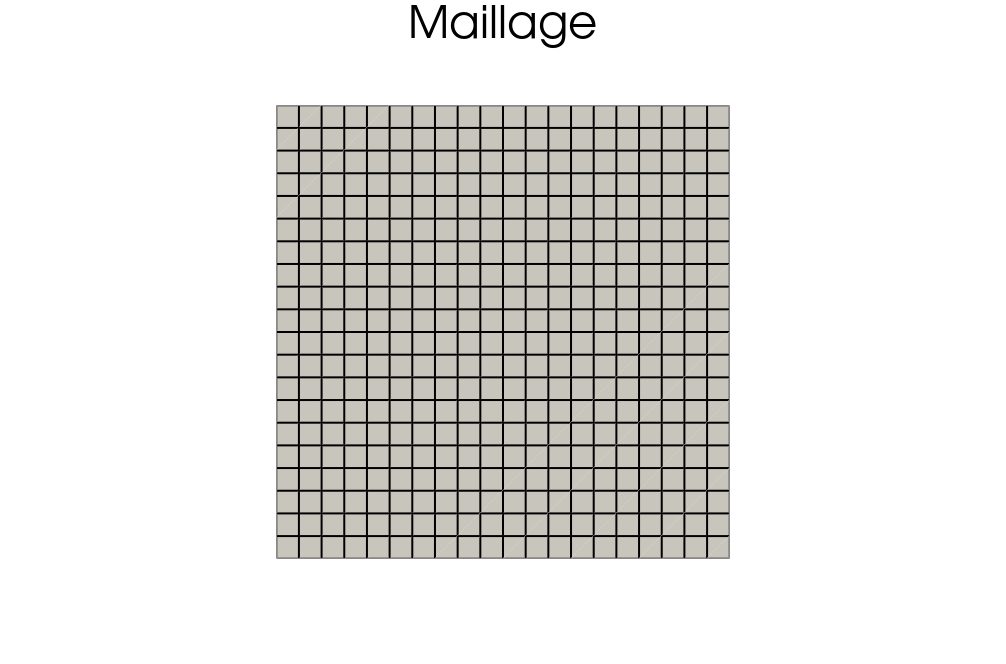
\includegraphics[width=\textwidth]{maillage_quad.png}
 	\caption{Maillage quadrilatère}
	\label{mesh_quad}
\end{figure}

\begin{figure}
	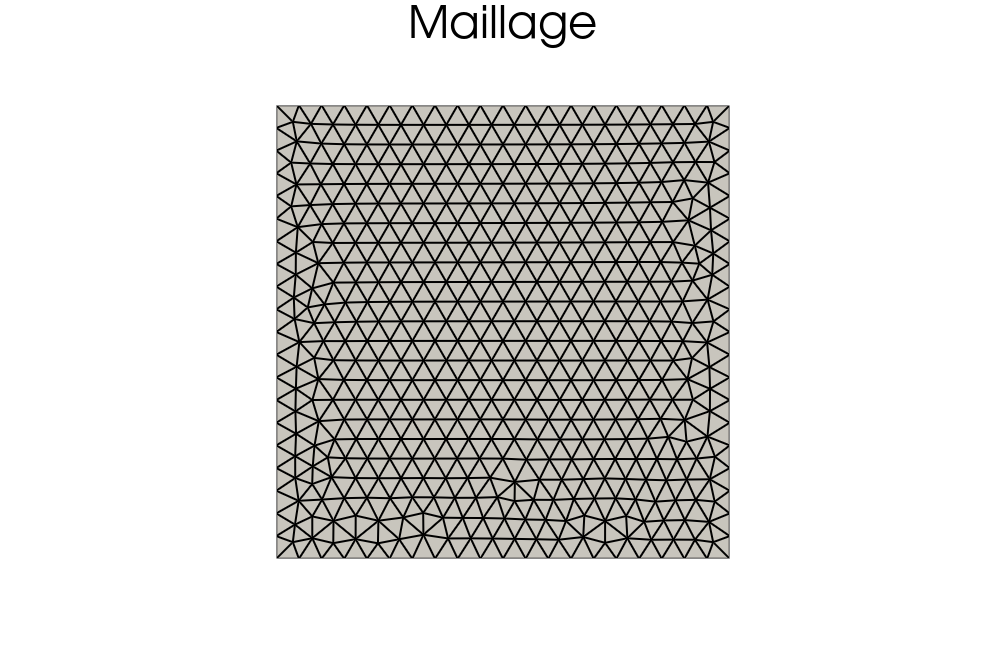
\includegraphics[width=\textwidth]{maillage_tri.png}
	\caption{Maillage triangulaire}
	\label{mesh_tri}
\end{figure}

\section{Résultats}

\subsection{Validation avec MMS}

\begin{figure}
	\begin{subfigure}[t]{0.48\textwidth}
		\includegraphics[width=\textwidth]{mms_upwind_quad_field_k1.pdf}
		\caption{Solution MMS avec schéma upwind vs solution numérique}
	\end{subfigure}
	\hfill
	\begin{subfigure}[t]{0.48\textwidth}
		% \includegraphics[width=\textwidth]{../figures/mms_rms_tri_cross.pdf}
		\includegraphics[width=\textwidth]{mms_upwind_quad_rms_k1.pdf}
		\caption{Convergence observée avec schéma upwind à l'aide de
		l'erreur RMS (Ordre de convergence: 0.9071)}
	\end{subfigure}\\
	\begin{subfigure}[t]{0.48\textwidth}
		\includegraphics[width=\textwidth]{mms_centre_quad_field_k1.pdf}
		\caption{Solution MMS avec schéma centré vs solution numérique}
	\end{subfigure}
	\hfill
	\begin{subfigure}[t]{0.48\textwidth}
		% \includegraphics[width=\textwidth]{../figures/mms_rms_tri_cross.pdf}
		\includegraphics[width=\textwidth]{mms_centre_quad_rms_k1.pdf}
		\caption{Convergence observée avec schéma centré à l'aide de
		l'erreur RMS (Ordre de convergence: 2.00047)}
	\end{subfigure}
	\caption{Maillage quadrilatère avec diffusion croisée pour l'exemple MMS}
	\label{fig:MMS_quad_cd}
\end{figure}

\begin{figure}
	\begin{subfigure}[t]{0.48\textwidth}
		\includegraphics[width=\textwidth]{mms_upwind_tri_cd_field_k1.pdf}
		\caption{Solution MMS avec schéma upwind vs solution numérique}
	\end{subfigure}
	\hfill
	\begin{subfigure}[t]{0.48\textwidth}
		% \includegraphics[width=\textwidth]{../figures/mms_rms_tri_cross.pdf}
		\includegraphics[width=\textwidth]{mms_upwind_tri_cd_rms_k1.pdf}
		\caption{Convergence observée avec schéma upwind à l'aide de
		l'erreur RMS (Ordre de convergence: 0.98812)}
	\end{subfigure}\\
	\begin{subfigure}[t]{0.48\textwidth}
		\includegraphics[width=\textwidth]{mms_centre_tri_cd_field_k1.pdf}
		\caption{Solution MMS avec schéma centré vs solution numérique}
	\end{subfigure}
	\hfill
	\begin{subfigure}[t]{0.48\textwidth}
		\includegraphics[width=\textwidth]{mms_centre_tri_cd_rms_k1.pdf}
		\caption{Convergence observée avec schéma centré à l'aide de
		l'erreur RMS (Ordre de convergence: 2.04008)}
	\end{subfigure}
	\caption{Maillage triangulaire sans diffusion croisée pour l'exemple MMS}
	\label{fig:MMS_tri_no_cd}
\end{figure}

\subsection{Versteeg Exemple 5.1i)}

\begin{figure}
	\begin{subfigure}[t]{0.48\textwidth}
		\includegraphics[width=\textwidth]{ex5_1i_quad_nocd_upwind.pdf}
		\caption{Solution analytique vs solution numérique avec un
		schéma centré sur une coupe à $Y=H/2$}
	\end{subfigure}
	\hfill
	\begin{subfigure}[t]{0.48\textwidth}
		\includegraphics[width=\textwidth]{epsilon5_1i_quad_nocd_upwind.pdf}
		\caption{Convergence observée pour schéma centré à l'aide de
		l'erreur RMS (0.95231)}
	\end{subfigure} \\
	\begin{subfigure}[t]{0.48\textwidth}
		\includegraphics[width=\textwidth]{ex5_1i_quad_nocd_centre.pdf}
		\caption{Solution analytique vs solution numérique avec un
		schéma centré sur une coupe à $Y=H/2$}
	\end{subfigure}
	\hfill
	\begin{subfigure}[t]{0.48\textwidth}
		\includegraphics[width=\textwidth]{epsilon5_1i_quad_nocd_centre.pdf}
		\caption{Convergence observée pour schéma centré à l'aide de
		l'erreur RMS (1.96118)}
	\end{subfigure}
	\caption{Maillage quadrilatère pour l'exemple 5.1i)}
\end{figure}

\begin{figure}
	\begin{subfigure}[t]{0.48\textwidth}
		\includegraphics[width=\textwidth]{ex5_1i_tri_cd_upwind.pdf}
		\caption{Solution analytique vs solution numérique avec un
		schéma centré sur une coupe à $Y=H/2$}
	\end{subfigure}
	\hfill
	\begin{subfigure}[t]{0.48\textwidth}
		\includegraphics[width=\textwidth]{epsilon5_1i_tri_cd_upwind.pdf}
		\caption{Convergence observée pour schéma centré à l'aide de
		l'erreur RMS (0.93727)}
	\end{subfigure} \\
	\begin{subfigure}[t]{0.48\textwidth}
		\includegraphics[width=\textwidth]{ex5_1i_tri_cd_centre.pdf}
		\caption{Solution analytique vs solution numérique avec un
		schéma centré sur une coupe à $Y=H/2$}
	\end{subfigure}
	\hfill
	\begin{subfigure}[t]{0.48\textwidth}
		\includegraphics[width=\textwidth]{epsilon5_1i_tri_cd_centre.pdf}
		\caption{Convergence observée pour schéma centré à l'aide de
		l'erreur RMS (1.7683)}
	\end{subfigure}
	\caption{Maillage triangulaire pour l'exemple 5.1i)}
\end{figure}


\subsection{Maillage quadrilatère transfini}

Le maillage utilisé est un carré de 2x2 composé de 20 éléments selon x et y, il est présenté en figure~\ref{xxxx}.

Afin de faire varier le nombre de Peclet nous avons fait varier la conductivité thermique $k$.

AJOUTER les savefig dans le code pour les contours et les coupes à x et y constants.

AJOUTER ordres de convergence 

\begin{figure}
	\begin{subfigure}[t]{0.3\textwidth}
		\includegraphics[width=\textwidth]{../figures/contours_quad_centre_k1.pdf}
		\caption{Contours des champs de température}
	\end{subfigure}
	\hfill
	\begin{subfigure}[t]{0.3\textwidth}
		\includegraphics[width=\textwidth]{../figures/XXXXX.pdf}
		\caption{Coupe à $Y = 1$}
	\end{subfigure}
	\hfill
	\begin{subfigure}[t]{0.3\textwidth}
		\includegraphics[width=\textwidth]{../figures/mms_centre_quad_rms_k1.pdf}
		\caption{Convergence observée à l'aide de l'erreur RMS}
	\end{subfigure}
	\caption{Maillage quadrilatère, méthode centrée pour $k = 1$}
	\label{fig:quad_centre_k1}
\end{figure}

RÉPÉTER POUR TOUS LES K PUIS PAREIL EN CENTRÉ

\subsection{Maillage triangulaire}



\printbibliography[]
	

\end{document}
